\chapter{Agenti risolutori di problemi}
Adottano il paradigma della \textbf{risoluzione di problemi come ricerca in uno spazio di stati} (\textit{problem solving}).\
Sono agenti \textbf{con modello} (storia percezioni) che adottano una rappresentazione atomica dello stato.\
Sono particolari \textbf{agenti con obiettivo}, che pianificano l'intera sequenza di mosse prima di agire.

\subsubsection{Il processo di risoluzione}
Passi da seguire:
\begin{enumerate}
	\item Determinazione obiettivo (un insieme di stati in cui obiettivo è soddisfatto)
	\item  Formulazione del problema
	      \begin{itemize}
		      \item rappresentazione degli stati
		      \item rappresentazione delle azioni
	      \end{itemize}
	\item Determinazione della soluzione mediante \textbf{ricerca} (un piano)
	\item Esecuzione del piano
\end{enumerate}

\subsubsection{Che tipo di assunzioni?}
L'ambiente è statico, osservabile (so dove sono), discreto (un insieme finito di azioni possibili) e deterministico (1 azione $\rightarrow$ 1 risultato).\
Si assume che l'agente possa eseguire il piano ``ad occhi
chiusi'', niente può andare storto.

\subsubsection{Formulazione del problema}
Un problema può essere definito formalmente mediante cinque componenti:

\begin{enumerate}
	\item Stato iniziale
	\item Azioni possibili in \textit{s}:\ Azioni(\textit{s})
	\item Modello di transizione:
	      \begin{itemize}
		      \item Risultato: $stato \times azione \rightarrow stato$
		      \item Risultato(s, a) = s', uno stato \textbf{successore}
	      \end{itemize}
	\item Test obiettivo:
	      \begin{itemize}
		      \item Un insieme di stati obiettivo
		      \item Goal-Test: $stato \rightarrow \{true, false\}$
	      \end{itemize}
	\item Costo del cammino
	      \begin{itemize}
		      \item somma dei costi delle azioni (costo dei passi)
		      \item costo di passo:\ c(s, a, s')
		      \item Il costo di un'azione/passo non è mai negativo
	      \end{itemize}
\end{enumerate}
1, 2 e 3 definiscono implicitamente lo spazio degli stati (definirlo esplicitamente può essere molto oneroso, come in quasi tutti i problemi di IA, questo sarà rilevante nel seguito).

\section{Algoritmi di ricerca}
\begin{center}
	``\textit{Il processo che cerca una sequenza di azioni che raggiunge l'obiettivo è detto \textbf{ricerca}}''
\end{center}
Gli algoritmi di ricerca prendono in input un problema e restituiscono un \textbf{cammino soluzione}, i.e. un cammino che porta dallo stato iniziale a uno stato goal.

\textit{Misura delle prestazioni}:\ Trova una soluzione?\ Quanto costa trovarla?\
Quanto efficiente è la soluzione?

\[ \mathrm{Costo\ totale = costo\ della\ ricerca + costo\ del\ cammino\ soluzione}\]

\subsection{Itinerario: il problema}
Trovare il percorso più breve da una città di partenza a una città di arrivo.
\begin{figure}[H]
	\centering
	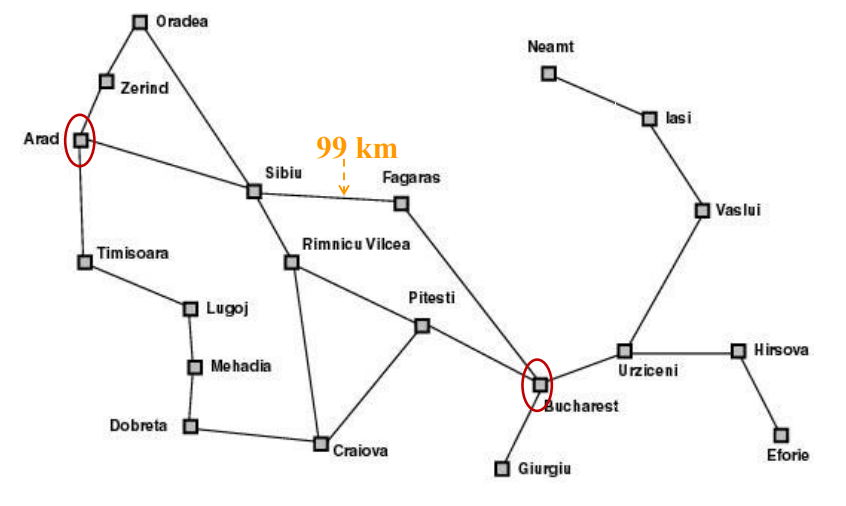
\includegraphics[width=0.9\textwidth]{immagini/Itinerario.png}
\end{figure}

\subsubsection{Formulazione}

\textit{Stati}:\ le città.
\begin{enumerate}
	\item \textit{Stato iniziale}:\ la città da cui si parte.\ \textit{In}(Arad)
	\item \textit{Azioni}:\ spostarsi su una città vicina collegata.\\ Azioni(\textit{In}(Arad)) = \{\textit{Go}(Sibiu), \textit{Go}(Zerind) \dots \}
	\item \textit{Modello di transizione}:\ Risultato(\textit{In}(Arad), \textit{Go}(Sibiu)) = \textit{In}(Sibiu)
	\item Test Obiettivo:\ \{\textit{In}(Bucarest)\}
	\item \textit{Costo del cammino}:\ somma delle lunghezze delle strade
\end{enumerate}
Lo \textbf{spazio degli stati} coincide con la rete (grafo) di collegamenti tra città i.e.\ grafo di stati collegati da azioni, rappresentabile in modo esplicito in questo caso semplice, tramite la mappa.

Astrazione dai dettagli:\ essenziale per ``modellare''.
\newpage
\subsection{Aspirapolvere: il problema (toy problem)}
Versione semplice:\ solo due locazioni, sporche o pulite, l'agente può essere in una delle due.

\begin{figure}[H]
	\centering
	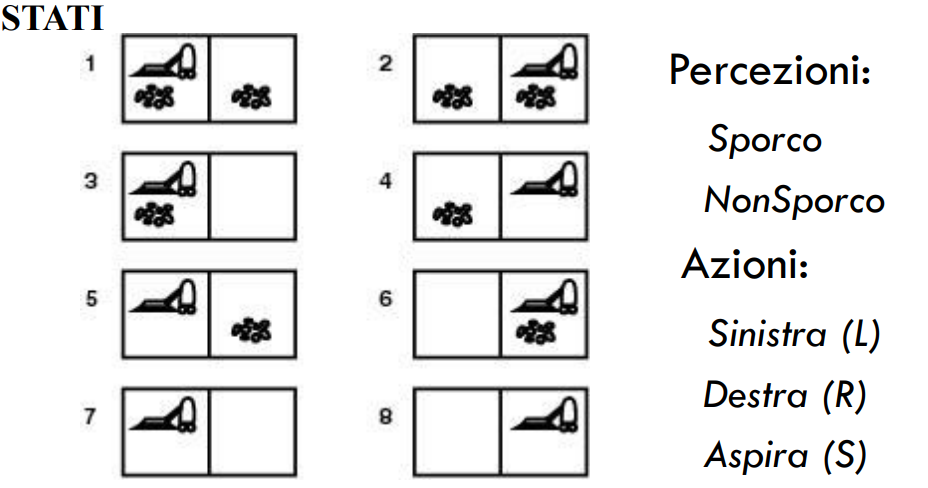
\includegraphics[width=0.8\textwidth]{immagini/Aspirapolvere.png}
\end{figure}
\subsubsection{Formulazione}
\textit{Obiettivo}:\ rimuovere lo sporco \{7, 8\}.\
Ogni azione ha costo 1.
\begin{figure}[H]
	\centering
	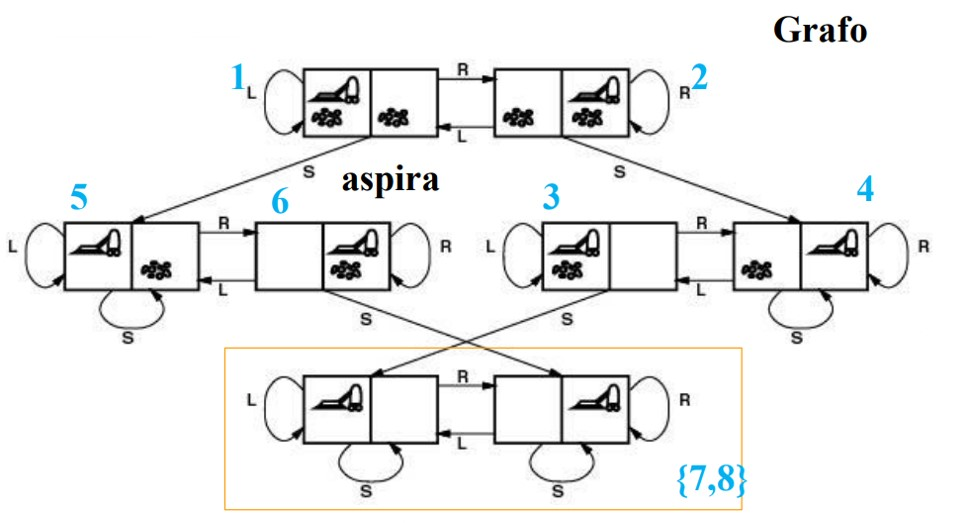
\includegraphics[width=0.8\textwidth]{immagini/Aspirapolvere_formulazione.jpg}
\end{figure}

\subsection{Il puzzle dell'otto}

\begin{figure}[H]
	\centering
	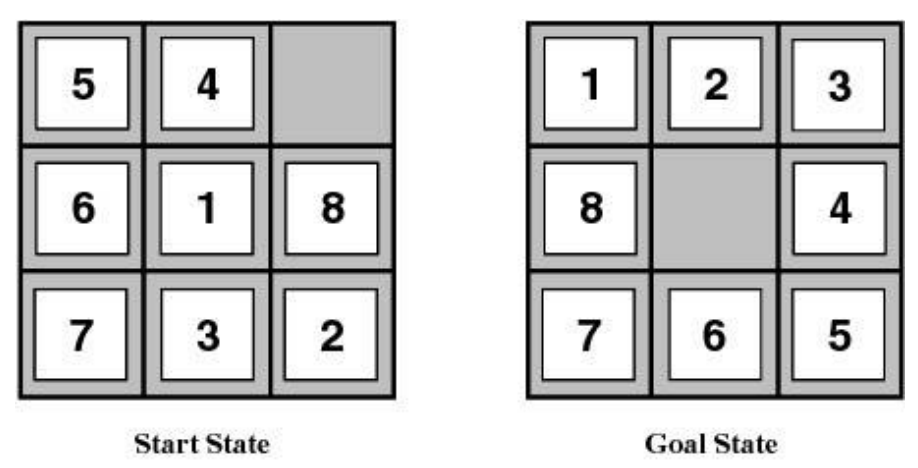
\includegraphics[width=0.6\textwidth]{immagini/Puzzle_otto.png}
\end{figure}

\subsubsection{Formulazione}
\begin{itemize}
	\item \textit{Stati}:\ possibili configurazioni della scacchiera.
	\item \textit{Azioni}:\ mosse della casella bianca
	      \begin{table}[H]
		      \centering
		      \begin{tabular}{l l}
			      in sù: $\uparrow$       & in giù: $\downarrow$     \\
			      a destra: $\rightarrow$ & a sinistra: $\leftarrow$ \\
		      \end{tabular}
	      \end{table}
	\item \textit{Costo cammino}:\ ogni passo costa 1
\end{itemize}
Lo spazio degli stati è un grafo con possibili cicli.\
NP-completo.\
Per 8 tasselli:\ 9!/2 = 181K stati! Ma risolvibile in poco tempo (ms).\
Se cresce no!

\subsection{Le otto regine: il problema }

Collocare otto regine sulla scacchiera in modo tale che nessuna regina sia attaccata da altre.
\begin{figure}[H]
	\centering
	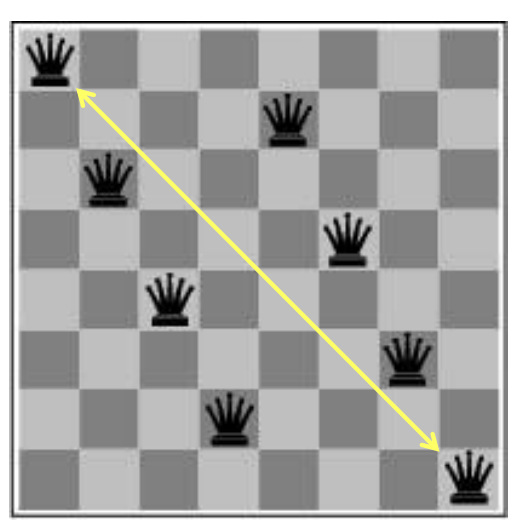
\includegraphics[width=0.4\textwidth]{immagini/otto_regine.png}
\end{figure}

\subsubsection{Formulazione incrementale 1}
Si aggiungono le regine una alla volta.

\begin{itemize}
	\item \textit{Stati}:\ scacchiere con 0-8 regine
	\item \textit{Goal-Test}:\ 8 regine sulla scacchiera, nessuna attaccata
	\item \textit{Costo cammino}:\ zero (resta 8 per le 8 mosse effettive e non è rilevante, interessa solo lo stato finale)
	\item \textit{Azioni}:\ aggiungi una regina
	\item \textit{Spazio stati}:\ 64 $\times$ 63 $\times$ \dots $\times$ 57 $\sim$ 1.8 $\times$ 10\textsuperscript{14} sequenze possibili da considerare!
\end{itemize}
La ricerca può essere molto onerosa!

\subsubsection{Formulazione incrementale 2}
\begin{itemize}
	\item \textit{Stati}:\ scacchiere con 0-8 regine, \textbf{nessuna minacciata}
	\item \textit{Goal-Test}:\ 8 regine sulla scacchiera, nessuna minacciata
	\item \textit{Costo cammino}:\ zero
	\item \textit{Azioni}:\ aggiungi una regina n\textbf{ella colonna vuota più a destra ancora libera in modo che non sia minacciata}.
\end{itemize}
2057 sequenze da considerare.

\subsubsection{Formulazione a stato completo}
\begin{itemize}
	\item \textit{Stati}:\ 8 regine già sulla scacchiera, nessuna minacciata
	\item \textit{Costo cammino}:\ zero
	\item \textit{Stati}:\ scacchiera con \textbf{8 regine, una per colonna}
	\item \textit{Azioni}:\ \textbf{sposta una regina nella colonna, se minacciata}
\end{itemize}

\subsection{Dimostrazione di teoremi}
Il problema:\ dato un insieme di premesse
\[
	\{s, t, q \Rightarrow p, r \Rightarrow p, v \Rightarrow q, t \Rightarrow r, s \Rightarrow v\}
\]
\textit{dimostrare una proposizione p}.\
Nel calcolo proposizionale un'unica regola di inferenza, il Modus Ponens (MP):

\[\mathrm{Se}\ p\ \mathrm{e}\ p \Rightarrow q\ \mathrm{allora}\ q.\]


\subsubsection{Dimostrazione teoremi: formulazione}

\begin{itemize}
	\item \textit{Stati}:\ insiemi di proposizioni
	\item \textit{Stato iniziale}:\ un insieme di proposizioni (le premesse).
	\item \textit{Stato obiettivo}:\ un insieme di proposizioni contenente il teorema da dimostrare.
	\item \textit{Operatori}:\ l'applicazione del MP, che aggiunge teoremi.
\end{itemize}

\begin{figure}[H]
	\centering
	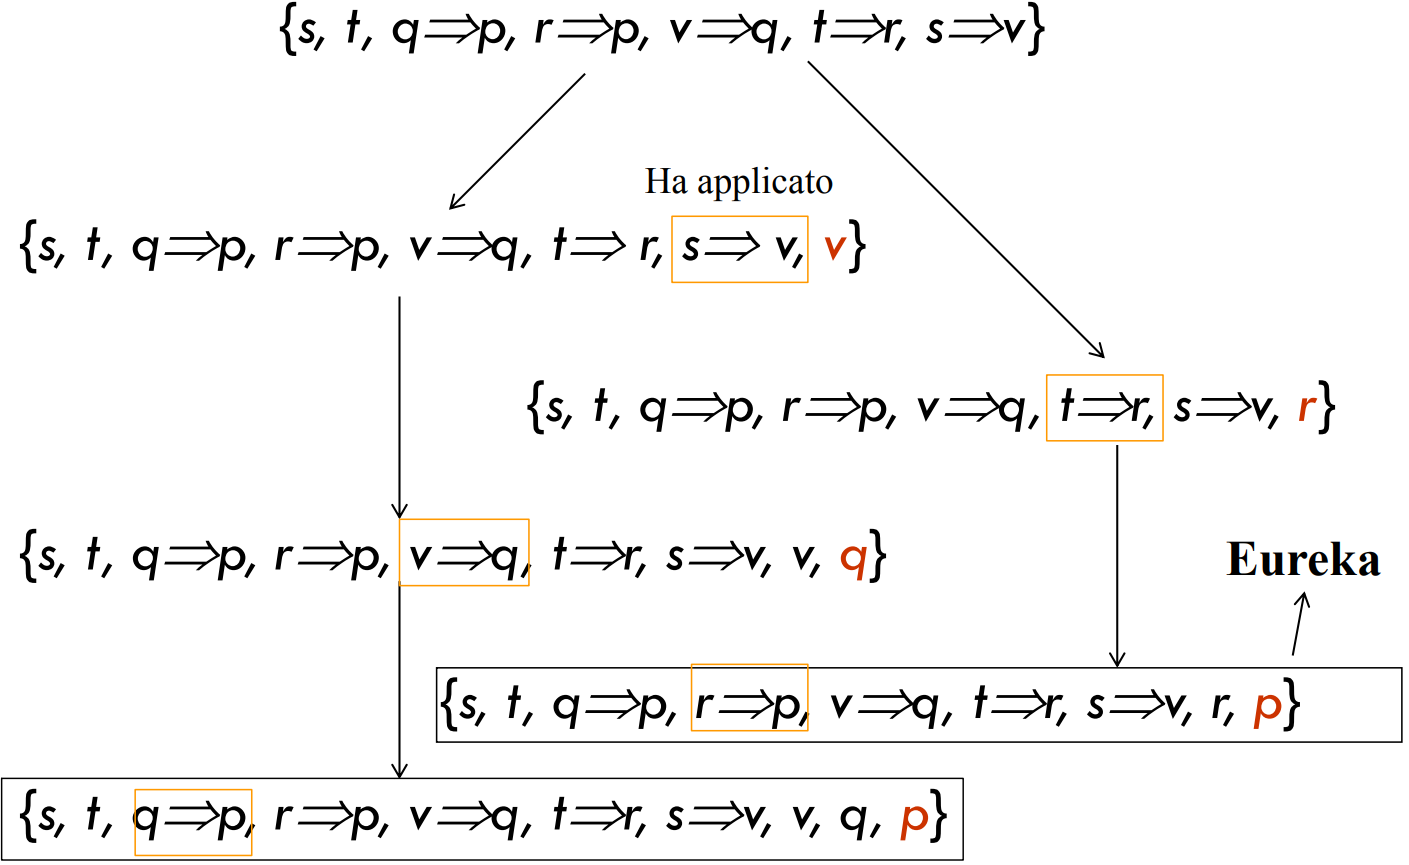
\includegraphics[width=0.7\textwidth]{immagini/Dim_teoremi.png}
\end{figure}

\subsection{Problemi reali}

Pianificazione di viaggi aerei
\begin{itemize}
	\item Problema del commesso viaggiatore
	\item Configurazione VLSI
	\item Navigazione di robot (spazio continuo!)
	\item Montaggio automatico
	\item Progettazione di proteine
	\item \dots
\end{itemize}

\section{Ricerca della soluzione}
Generazione di un \textbf{albero di ricerca} sovrapposto allo \textbf{spazio degli stati} (generato da \textit{possibili} sequenze di azioni).

La \textbf{ricerca} è approfondire un'opzione, tenendo da parte le altre per poi ripredenderle se non si trova una soluzione.
\begin{figure}[H]
	\centering
	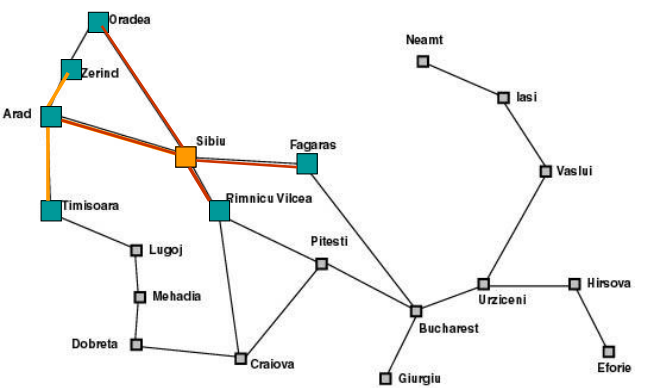
\includegraphics[width=0.7\textwidth]{immagini/albero_ricerca.png}
\end{figure}

Generazione di un \textit{albero di ricerca} sovrapposto allo spazio degli stati.

\begin{figure}[H]
	\centering
	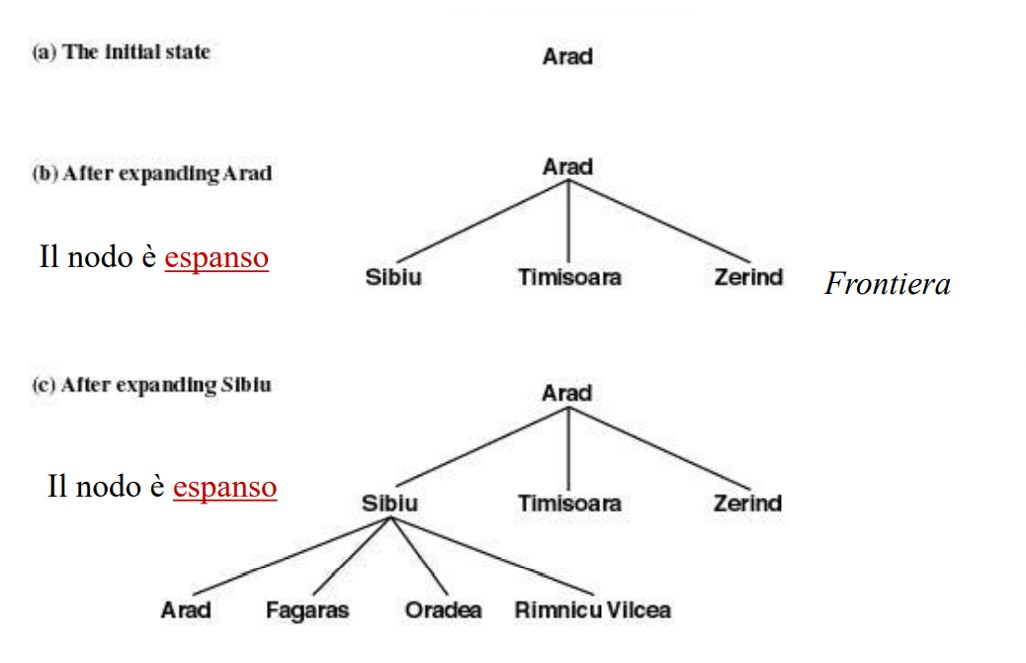
\includegraphics[width=0.8\textwidth]{immagini/generazione_albero_ricerca.jpg}
\end{figure}

\noindent\textbf{Nota}:\ ``nodo'' diverso da ``stato'', per esempio possono esistere esistono nodi di un albero di ricerca con stesso stato (città).

\subsection{Ricerca ad albero}
Ossia senza controllare se i nodi (stati) siano già stati esplorati.\
Vedremo la ricerca ``a/su grafo'' con questi controlli.
\begin{flushleft}
	\textbf{function} Ricerca-Albero (\textit{problema}) \textbf{returns} \textit{soluzione} oppure \textit{fallimento}

	\quad Inizializza la frontiera con stato iniziale del problema

	\quad \textbf{loop do}

	\quad \qquad \textbf{if} \textit{la frontiera è vuota} \textbf{then return}  \textit{fallimento}

	\quad \qquad \textit{Scegli un nodo foglia da espandere e rimuovilo dalla  frontiera}

	\quad \qquad \textbf{if} \textit{il nodo contiene uno stato obiettivo}

	\quad \qquad \quad \textbf{then return} \textit{soluzione corrispondente}

	\quad \qquad \textit{Espandi il nodo e aggiungi i successori alla frontiera}

	\quad \end{flushleft}

\subsection{I nodi dell'albero di ricerca}

Un nodo \textit{n} è una struttura dati con quattro componenti:\ uno stato, \textit{n}.stato, il nodo padre, \textit{n}.padre, l'azione effettuata per generarlo, \textit{n}.azione, e il costo del cammino dal nodo iniziale al nodo, N.costo-cammino indicata come $g(n)$ (= \textit{padre.costo-cammino} + \textit{costo-passo ultimo}).

\subsection{Struttura dati per la frontiera}

\textbf{Frontiera}:\ lista dei nodi in attesa di essere espansi (le foglie dell'albero di ricerca).\
La frontiera è implementata come una coda con operazioni:
\begin{itemize}
	\item Vuota?(coda)
	\item POP(coda) estrae il primo elemento
	\item Inserisci(elemento, coda)
	\item Diversi tipi di coda hanno diverse funzioni di inserimento e implementano \textit{strategie} diverse
\end{itemize}

\subsection{Diversi tipi di strategie (di ricerca)}

\begin{itemize}
	\item FIFO - First In First Out $\rightarrow$ BF:\ viene estratto l'elemento più vecchio (in attesa da più tempo); i nuovi nodi sono aggiunti alla fine.
	\item LIFO - Last In First Out $\rightarrow$ DF:\ viene estratto il più recentemente inserito; i nuovi nodi sono inseriti all'inizio.
	\item Coda con priorità $\rightarrow$ UC, et altri successivi:\ viene estratto quello con priorità più alta in base a una funzione di ordinamento; dopo l'inserimento dei nuovi nodi si riordina.
\end{itemize}

\subsubsection{Strategie non informate}
\begin{itemize}
	\item Ricerca in ampiezza (BF)
	\item Ricerca in profondità (DF)
	\item Ricerca in profondità limitata (DL)
	\item Ricerca con approfondimento iterativo (ID)
	\item Ricerca di costo uniforme (UC)
\end{itemize}
Tali strategie verranno confrontate con strategie di ricerca euristica (o informata):\ fanno uso di informazioni riguardo alla distanza stimata dalla soluzione.

\subsection{Valutazione di una strategia}

\begin{itemize}
	\item \textit{Completezza}:\ se la soluzione esiste viene trovata
	\item \textit{Ottimalità} (ammissibilità):\ trova la soluzione migliore, con costo minore (per il ``costo del cammino soluzione'')
	\item \textit{Complessità in tempo}:\ tempo richiesto per trovare la soluzione
	\item \textit{Complessità in spazio}:\ memoria richiesta
\end{itemize}
Quest'ultimi due fattori riguardono il ``costo della ricerca''.

\subsection{Ricerca in ampiezza (BF - Breadth-first)}
Consiste nell'esplorare il grafo dello spazio degli stati a livelli progressivi di stessa profondità.\
Implementata con una coda che inserisce alla fine (\textbf{FIFO}).\

\subsubsection{Ricerca in ampiezza ad albero}
Senza gestire problema stati già esplorati.

\begin{flushleft}
	\textbf{function} Ricerca-Ampiezza-A (\textit{problema}) \textbf{returns} soluzione oppure \textbf{fallimento}

	\quad \textit{nodo} = un nodo con \textit{stato il problema.stato-iniziale e}

	\qquad \textit{costo-di-cammino=0}

	\quad \textbf{if} \textit{problema}.\textit{Test-Obiettivo}(\textit{nodo}.Stato) \textbf{then return} Soluzione(\textit{nodo})

	\quad \textit{frontiera} = una coda FIFO con \textit{nodo} come unico elemento

	\quad \textbf{loop do}

	\quad \quad \textbf{if} \textit{Vuota?(frontiera)} \textbf{then return fallimento}

	\quad \quad \textit{nodo} = POP(\textit{frontiera})

	\quad \quad \textbf{for each} azione \textbf{in} problema.Azioni(\textit{nodo}.Stato) \textbf{do}

	\quad \qquad \textit{figlio} = Nodo-Figlio(\textit{problema}, \textit{nodo}, \textit{azione})

	\quad \qquad \textbf{if} \textit{problema}.\textit{TestObiettivo}(\textit{figlio}.Stato) \textbf{then return} Soluzione(\textit{figlio})

	\quad \qquad \textit{frontiera} = Inserisci(\textit{figlio}, \textit{frontiera})

	\quad \noindent end
\end{flushleft}

\subsubsection{Ricerca in ampiezza su grafo}
Senza gestire problema stati già esplorati.

\begin{flushleft}
	\textbf{function} Ricerca-Ampiezza-A (\textit{problema}) \textbf{returns} soluzione oppure \textbf{fallimento}

	\quad \textit{nodo} = un nodo con \textit{stato il problema.stato-iniziale e}

	\quad \textit{costo-di-cammino=0}

	\quad \textbf{if} \textit{problema}.\textit{Test-Obiettivo}(\textit{nodo}.Stato) \textbf{then return} Soluzione(\textit{nodo})

	\quad \textit{frontiera} = una coda FIFO con \textit{nodo} come unico elemento

	\quad \textit{esplorati} = insieme vuoto

	\quad \textbf{loop do}

	\qquad \textbf{if} \textit{Vuota?(frontiera)} \textbf{then return fallimento}

	\qquad \textit{nodo} = POP(\textit{frontiera}); aggiungi \textit{nodo}.Stato a \textit{esplorati}

	\qquad \textbf{for each} azione \textbf{in} problema.Azioni(\textit{nodo}.Stato) \textbf{do}

	\qquad \quad \textit{figlio} = Nodo-Figlio(\textit{problema}, \textit{nodo}, \textit{azione})

	\qquad \quad \textbf{if} \textit{figlio}.Stato non è in \textit{esplorati} e non è in \textit{frontiera} \textbf{then}

	\qquad \qquad \textbf{if} \textit{problema}.\textit{TestObiettivo}(\textit{figlio}.Stato) \textbf{return} Soluzione(\textit{figlio})

	\qquad \qquad \textit{frontiera} = Inserisci(\textit{figlio}, \textit{frontiera})

	end
\end{flushleft}

\noindent Nota che in entrambe le versioni i \textit{nodo}.Stato sono goal-tested al momento in cui sono generati.\ $\rightarrow$ \textbf{Più efficiente}, si ferma appena trova goal prima di espandere.

\subsubsection{Analisi complessità spazio-temporale (BF)}

\begin{flushleft}
	Assumiamo:\

	\textbf{\textit{b}} = fattore di ramificazione (\textbf{b}ranching) (numero max di successori)

	\textbf{\textit{d}} = profondità del nodo obiettivo più superficiale (\textbf{d}epth) (più vicino all'iniziale)

	\textbf{\textit{m}} = lunghezza massima dei cammini nello spazio degli stati (\textbf{m}ax)
\end{flushleft}

\noindent È una strategia \textit{completa} ed è anche \textit{ottimale} \textbf{se gli operatori hanno tutti lo stesso costo \textit{k}}, cioè $g(n) = k \cdot depth(n)$, dove $g(n)$ è il costo del
cammino per arrivare a \textit{n}.
\begin{flushleft}
	Complessità nel tempo (nodi generati):
	\[T(b, d) = b + b^2 + \dots + b^d \rightarrow O(b^d)\]
\end{flushleft}

\noindent\textbf{Nota bene}:\ il numero nodi cresce esponenzialmente, non assumiamo di conoscere già il grafo né una notazione di linearità nel numero nodi.\
Questo è tipico dei problemi in AI (pensate a quelli generati per le configurazioni dei giochi, con rappresentazione implicita dello spazio stati).

\begin{flushleft}
	Complessità spazio (nodi in memoria):\ $O(b^d)$ (solo per la frontiera)

\end{flushleft}

\subsection{Ricerca in profondità (DF)}

Implementata da una coda che mette i successori in testa alla lista (LIFO, pila o stack).

Cancelli rami completamente esplorati ma tiene tutti i fratelli del path corrente:\ memoria solo $b \times m$.

\subsubsection{Ricerca in profondità: analisi (versione su albero)}

Se \textit{m} lunghezza massima dei cammini nello spazio degli stati e \textit{b} è il fattore di diramazione

\begin{table}[H]
	\centering
	\begin{tabular}{l}
		Tempo:\ $O(b^m)$, che può essere $> O(b^d)$        \\
		Occupazione memoria:\ $bm$ (frontiera sul cammino) \\
	\end{tabular}
\end{table}

\noindent Strategia \textit{non completa} (loop) e \textit{non ottimale}.\
Drastico risparmio in memoria:
\begin{table}[H]
	\centering
	\begin{tabular}{l l l}
		BF & $d=16$ & 10 esabyte \\
		DF & $d=16$ & 156 Kbyte  \\
	\end{tabular}
\end{table}

\subsubsection{Ricerca in profondità: analisi (versione su grafo)}

In caso di DF con visita a grafo si perdono i vantaggi di memoria:\ la memoria torna da $b \times m$ a tutti i possibili stati (potenzialmente, caso pessimo, esponenziale come BF) (per mantenere la lista dei visitati/esplorati), ma cosi DF diviene completa in spazi degli stati finiti (tutti i nodi verranno espansi nel caso pessimo).\
Resta comunque non completa in spazi infiniti.\

Sarebbe possibile controllare anche solo i nuovi stati rispetto al cammino radice-nodo corrente senza aggravio di memoria evitando però cosi solo i cicli finiti in spazi finiti ma non i cammini ridondanti.

\subsubsection{Ricerca in profondità (DF) ricorsiva}

Ancora più efficiente in occupazione di memoria perché mantiene solo il cammino corrente (solo \textit{m} nodi nel caso pessimo).\
Realizzata da un algoritmo ricorsivo ``con backtracking'' che non necessita di tenere in memoria \textit{b} nodi per ogni livello, ma salva lo stato su uno stack a cui torna in caso di fallimento per fare altri tentativi.\

\begin{flushleft}
	\textbf{function} Ricerca-DF-A (\textit{problema}) \textbf{returns} soluzione oppure fallimento

	\quad return Ricerca-DF-ricorsiva(CreaNodo(\textit{problema}.Stato-iniziale),

	\qquad\textit{problema})
\end{flushleft}

\begin{flushleft}
	\textbf{function} Ricerca-DF-ricorsiva(\textit{nodo}, \textit{problema}) \textbf{returns} soluzione oppure \textbf{fallimento}

	\quad \textbf{if} \textit{problema}.TestObiettivo(\textit{nodo}.Stato) \textbf{then return} Soluzione(\textit{nodo})

	\quad else

	\quad \textbf{for each} \textit{azione} \textbf{in} \textit{problema}.Azioni(\textit{nodo}.Stato) \textbf{do}

	\quad \quad \quad \textit{figlio} = Nodo-Figlio(\textit{problema}, \textit{nodo}, \textit{azione})

	\qquad \quad \textit{risultato} = Ricerca-DF-ricorsiva(\textit{figlio}, \textit{problema})

	\qquad \quad \textbf{if} \textit{risultato} $\neq$ \textit{fallimento} \textbf{then return} \textit{risultato}

	\textbf{return fallimento}
\end{flushleft}

\subsubsection{Ricerca in profondità limitata (DL)}
Si va in profondità fino ad un certo livello predefinito \textit{l}.\
Completa per problemi in cui si conosce un limite superiore per la profondità della soluzione.

È completo se $d < l$, ma non è ottimale.\
\begin{center}
	Complessità tempo:\ $O(b^l)$

	Complessità spazio:\ $O(bl)$
\end{center}

\subsection{Approfondimento iterativo (ID)}

\begin{figure}[H]
	\centering
	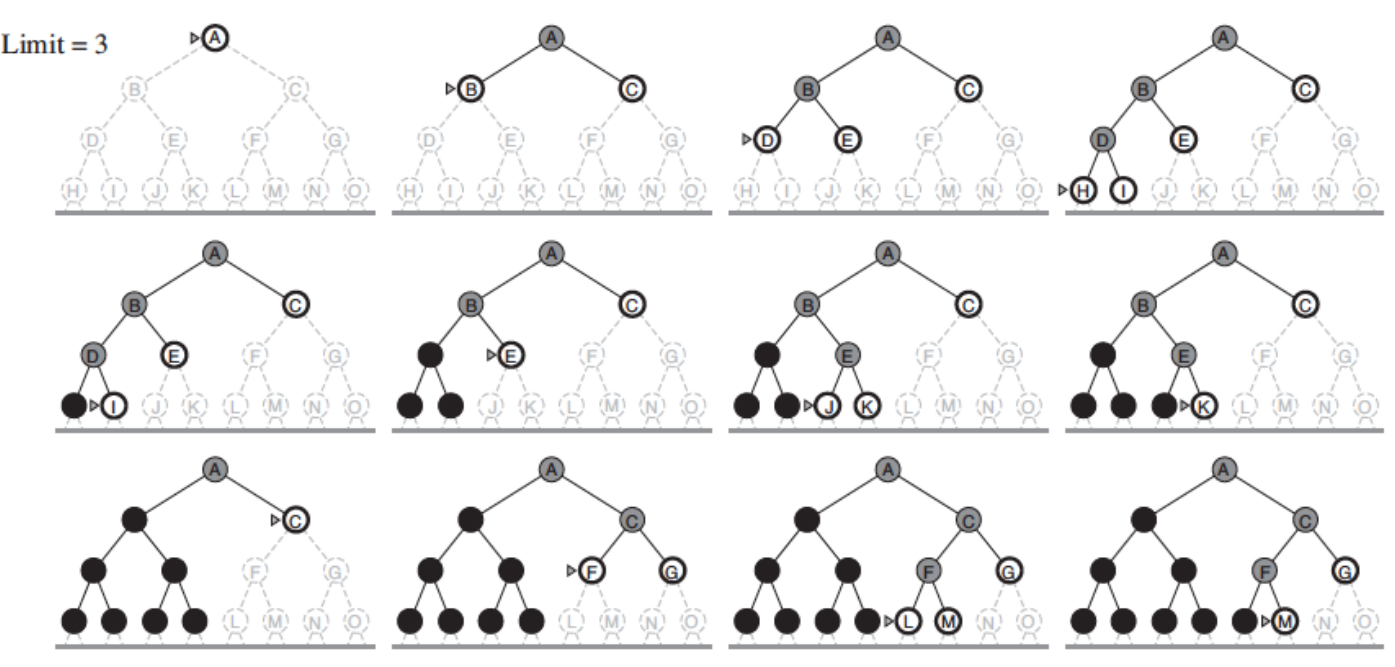
\includegraphics[width=\textwidth]{immagini/Approfondimento_iterativo.png}
\end{figure}

Miglior compromesso tra BF e DF
\[\mathrm{BF}:\ b+b^2+ \dots +b^{d-1}+b^d\]
con $b=10$ e $d=5$
\[10+100+1000+10.000+100.000=111.110\]
ID: I nodi dell'ultimo livello generati una volta, quelli del penultimo 2, quelli del terzultimo 3 \dots quelli del primo \textit{d} volte.
\begin{center}
	ID:\ $(d)b+(d-1) b^2+ \dots +3b^{d-2}+2b^{d-1}+1b^d = 50+400+3000+20.000+100.000=123450$
\end{center}
\begin{center}
	Complessità tempo:\ $O(b^d)$

	Spazio:\ $O(bd)$ versus $O(b^d)$ della BF.
\end{center}
Ergo:\ vantaggi della BF, con tempi analoghi ma costo memoria analogo a quello di DF.

\subsection{Direzione della ricerca}

Un problema ortogonale alla strategia è la \textit{direzione della ricerca}.\
Nella ricerca \textbf{\textit{in avanti}} o \textit{guidata dai dati} si esplora lo spazio di ricerca dallo stato iniziale allo stato obiettivo; invece nella ricerca \textbf{\textit{all'indietro}} o \textbf{\textit{guidata dall'obiettivo}} si esplora lo spazio di ricerca a partire da uno stato goal e riconducendosi a sotto-goal fino a trovare uno stato iniziale.

Quale direzione scegliere?\ Conviene procedere nella direzione in cui il fattore di diramazione è minore.\ Si preferisce ricerca all'indietro quando:
\begin{itemize}
	\item l'obiettivo è chiaramente definito (e.g.\ theorem proving) o si possono formulare una serie limitata di ipotesi;
	\item i dati del problema non sono noti e la loro acquisizione può essere guidata dall'obiettivo.
\end{itemize}
Si preferisce ricerca in avanti quando:
\begin{itemize}
	\item gli obiettivi possibili sono molti (design);
	\item abbiamo una serie di dati da cui partire.
\end{itemize}
Nella ricerca bidirezionale si procede nelle due direzioni fino ad incontrarsi.\

\subsubsection{Ricerca bidirezionale: analisi}

Complessità tempo:\ $O(b^{d/2})$ (\slash2 = radice quadrata!)
(assumendo test intersezione in tempo costante, per esempio hash table).

\noindent Complessità spazio:\ $O(b^{d/2})$ (almeno tutti i nodi in una direzione in memoria, per esempio usando BF).

\textbf{Nota}:\ non sempre applicabile, per esempio nei casi di predecessori non definiti, troppi stati obiettivo\dots

\subsection{Ricerca ``ad albero''\slash``a grafo'':\ cammini ciclici}

I cammini ciclici rendono gli alberi di ricerca infiniti con spazi degli stati infiniti.\
Su spazi di stati a grafo si generano più volte gli stessi nodi (o meglio nodi con stesso stato) nella ricerca, \textbf{anche in assenza di cicli}.\

\subsubsection{Compromesso tra spazio e tempo}
Ricordare gli stati già visitati occupa spazio (ad esempio lista \textit{esplorati} in visita a grafo) ma ci consente di evitare di visitarli di nuovo.\

Gli algoritmi che dimenticano la propria storia sono destinati a ripeterla!

\subsubsection{Tre soluzioni}

In ordine crescente di costo e di efficacia:
\begin{itemize}
	\item Non tornare nello stato da cui si proviene:\ si elimina il genitore dai nodi successori (non evita i cammini ridondanti).
	\item Non creare cammini con cicli:\ si controlla che i successori non siano antenati del nodo corrente (detto per la DF).
	\item Non generare nodi con stati già visitati{\slash}esplorati:\ ogni nodo visitato deve essere tenuto in memoria per una complessità $O(s)$ dove \textit{s} è il numero di stati possibili (e.g.\ hash table per accesso efficiente).
\end{itemize}
\textit{Repetita}:\ il costo può essere alto; in caso di DF la memoria torna da $b \times m$ a tutti gli stati, ma diviene una ricerca completa (per spazi finiti).\
Ma in molti casi gli stati crescono in modo esponenziale (gioco otto, scacchi,\ \dots).

\subsubsection{Ricerca ``su grafi''}

Mantiene una lista dei nodi (stati) visitati/esplorati (anche detta \textbf{\textit{lista chiusa}}).\
Prima di espandere un nodo si controlla se lo stato era stato già incontrato prima o è già nella frontiera; se questo succede, il nodo appena trovato non viene
espanso.\

Ottimale solo se abbiamo la garanzia che il costo del nuovo cammino sia maggiore o uguale (cioè il nuovo cammino non conviene).

\subsection{Ricerca di costo uniforme (UC)}

Generalizzazione della ricerca in ampiezza (costi diversi tra passi):\ \textit{si sceglie il nodo di costo minore sulla frontiera} (si intende il costo $g(n)$ del cammino), si espande sui contorni di \textbf{uguale costo} (e.g.\ in km) invece che sui contorni di uguale profondità (BF).

\begin{figure}[H]
	\centering
	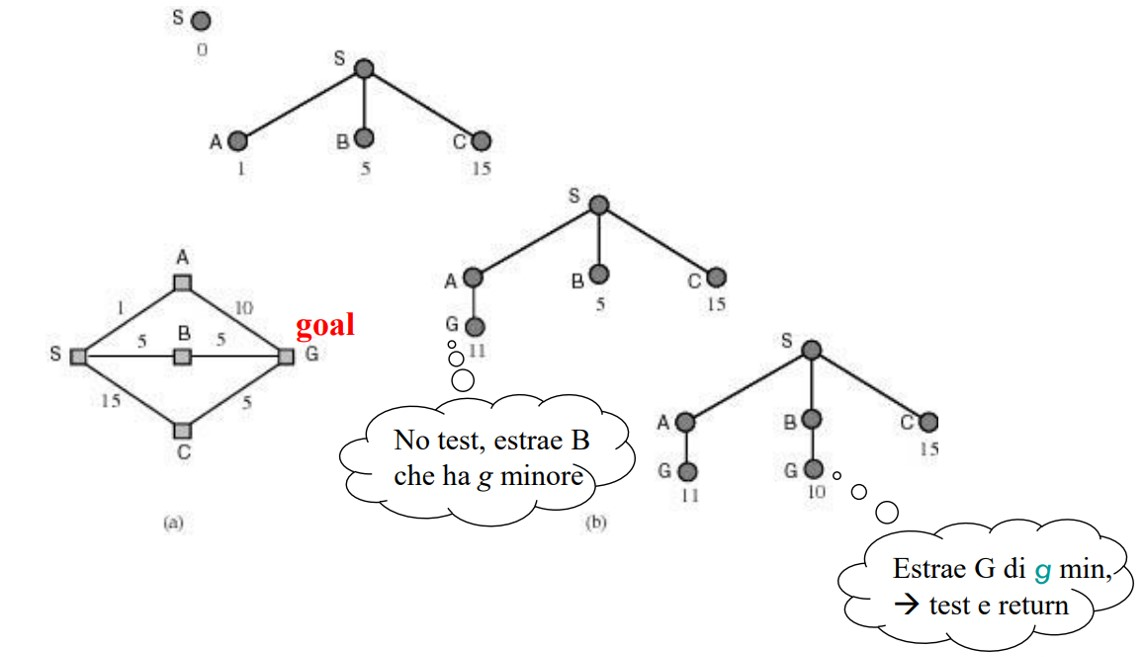
\includegraphics[width=\textwidth]{immagini/UC.jpg}
\end{figure}

\noindent Implementata da una coda ordinata per costo cammino crescente (in cima i nodi di costo minore).\

\subsubsection{Ricerca UC (su albero)}
\textbf{function} Ricerca-UC-A (\textit{problema}) \textbf{returns} soluzione oppure \textbf{fallimento}

\textit{nodo} = un nodo con \textit{stato il problema.stato-iniziale e costo-di-cammino=0}

\textit{frontiera} = una coda con priorità con \textit{nodo} come unico elemento

\textbf{loop do}
\quad \textbf{if} \textit{Vuota?}(\textit{frontiera}) \textbf{then return fallimento}

\quad \textit{nodo} = POP(\textit{frontiera})

\quad \textbf{if} \textit{problema}.TestObiettivo(\textit{nodo}.Stato) \textbf{then return} Soluzione(\textit{nodo})

\quad \textbf{for each} azione \textbf{in} \textit{problema}.Azioni(\textit{nodo}.Stato) \textbf{do}

\quad \quad  \textit{figlio} = Nodo-Figlio(\textit{problema}, \textit{nodo}, \textit{azione})

\quad \quad  \textit{frontiera} = Inserisci(\textit{figlio}, \textit{frontiera}) /* in coda con priorità

\textbf{end}

\subsubsection{Ricerca-grafo UC}

\textbf{function} Ricerca-UC-A (\textit{problema}) \textbf{returns} soluzione oppure \textbf{fallimento}

\textit{nodo} = un nodo con \textit{stato il problema.stato-iniziale e costo-di-cammino=0}

\textit{frontiera} = una coda con priorità con \textit{nodo} come unico elemento

\textit{esplorati} = insieme vuoto

\textbf{loop do}
\quad \textbf{if} \textit{Vuota?}(\textit{frontiera}) \textbf{then return fallimento}

\quad \textit{nodo} = POP(\textit{frontiera})

\quad \textbf{if} \textit{problema}.TestObiettivo(\textit{nodo}.Stato) \textbf{then return} Soluzione(\textit{nodo})

\quad aggiungi \textit{nodo}.Stato a \textit{esplorati}

\quad \textbf{for each} azione \textbf{in} \textit{problema}.Azioni(\textit{nodo}.Stato) \textbf{do}

\quad \quad  \textit{figlio} = Nodo-Figlio(\textit{problema}, \textit{nodo}, \textit{azione})

\quad \quad \textbf{if} \textit{figlio}.Stato non è in \textit{esplorati} e non è in \textit{frontiera} \textbf{then}

\qquad \quad  \textit{frontiera} = Inserisci(\textit{figlio}, \textit{frontiera}) /* in coda con priorità

\quad \quad \textbf{else if} \textit{figlio}.Stato è in \textit{frontiera} con Costo-cammino più alto \textbf{then}

\qquad \quad sostituisci quel nodo frontiera con figlio

\textbf{end}

\subsubsection{Analisi}

\textit{Ottimalità} e \textit{completezza} garantite purché il costo degli archi sia maggiore di $\varepsilon > 0$.

Assunto C* come il costo della soluzione ottima $\lfloor C^*/\varepsilon\rfloor$ è il numero di mosse nel caso peggiore, arrotondato per difetto (e.g.\ attratto ad andare verso tante mosse di costo $\varepsilon$ prima di una che parta più alta ma poi abbia un path a costo totale più basso).\

Complessità:\ $O(b^{1+\lfloor C^*/\varepsilon\rfloor})$.\
Si noti che quando ogni azione ha lo stesso costo UC somiglia a BF, ma ha complessità $O(b^{1+d})$ causata dall'esame e arresto posticipato:\ solo dopo aver espanso anche l’ultima frontiera, oltre la profondità del goal.

\subsection{Confronto delle strategie (albero)}

\begin{table}[H]
	\centering
	\begin{tabular}{|c|c|c|c|c|c|c|}
		\hline
		\textbf{Criterio} & \textbf{BF} & \textbf{UC}                               & \textbf{DF} & \textbf{DL} & \textbf{ID} & \textbf{Bidir} \\\hline
		Completa?         & sì          & sì ($\sim$)                               & no          & sì (+)      & sì          & sì             \\
		Tempo             & $O(b^d)$    & $O(b^{1+\lfloor C^*/\varepsilon\rfloor})$ & $O(b^m)$    & $O(b^l)$    & $O(b^d)$    & $O(b^{d/2})$   \\
		Spazio            & $O(b^d)$    & $O(b^{1+\lfloor C^*/\varepsilon\rfloor})$ & $O(bm)$     & $O(bl)$     & $O(bd)$     & $O(b^{d/2})$   \\
		Ottimale?         & sì (*)      & sì ($\sim$)                               & no          & no          & sì (*)      & sì             \\\hline
	\end{tabular}
\end{table}

\noindent(*) se gli operatori hanno tutti lo stesso costo.

\noindent($\sim$) per costi degli archi $ \geq \varepsilon > 0$.

\noindent(+) per problemi per cui si conosce un limite alla profondità della soluzione (se $l >d$).

\section{Conclusioni}
Un agente per ``problem solving'' adotta un paradigma generale di risoluzione dei problemi:\
\begin{itemize}
	\item formula il problema (parte non automatica),
	\item ricerca la soluzione nello spazio degli stati (diventa automatico).
\end{itemize}
Strategie ``non informate'' per la ricerca della soluzione.\

